% =====================================================================
% figC  — R/ggplot2 -> tikzDevice (parallel to ../figures-tex/figC_causal.tex)
% Canonical-JSON-only. Regenerate: Rscript figures/make_figures_ieee.R
% Provenance (JSON path :: field = plotted value), one line per series:
% SOURCE: results/C4_causal_table.json :: layers.8.quartile_means[cos=0.166].mean_damage_removed = 2.4138
% SOURCE: results/C4_causal_table.json :: layers.8.quartile_means[cos=0.261].mean_damage_removed = 3.7267
% SOURCE: results/C4_causal_table.json :: layers.8.quartile_means[cos=0.336].mean_damage_removed = 4.8788
% SOURCE: results/C4_causal_table.json :: layers.8.quartile_means[cos=0.464].mean_damage_removed = 6.2245
% SOURCE: results/C4_causal_table.json :: layers.10.quartile_means[cos=0.100].mean_damage_removed = 0.8223
% SOURCE: results/C4_causal_table.json :: layers.10.quartile_means[cos=0.167].mean_damage_removed = 1.3557
% SOURCE: results/C4_causal_table.json :: layers.10.quartile_means[cos=0.226].mean_damage_removed = 2.0480
% SOURCE: results/C4_causal_table.json :: layers.10.quartile_means[cos=0.362].mean_damage_removed = 3.6394
% SOURCE: results/C4_causal_table.json :: layers.12.quartile_means[cos=0.149].mean_damage_removed = 1.5718
% SOURCE: results/C4_causal_table.json :: layers.12.quartile_means[cos=0.236].mean_damage_removed = 2.3083
% SOURCE: results/C4_causal_table.json :: layers.12.quartile_means[cos=0.307].mean_damage_removed = 3.0652
% SOURCE: results/C4_causal_table.json :: layers.12.quartile_means[cos=0.447].mean_damage_removed = 4.7057
% SOURCE: results/C4_causal_table.json :: layers.14.quartile_means[cos=0.277].mean_damage_removed = 4.0476
% SOURCE: results/C4_causal_table.json :: layers.14.quartile_means[cos=0.379].mean_damage_removed = 4.8245
% SOURCE: results/C4_causal_table.json :: layers.14.quartile_means[cos=0.454].mean_damage_removed = 5.5521
% SOURCE: results/C4_causal_table.json :: layers.14.quartile_means[cos=0.590].mean_damage_removed = 6.8021
% SOURCE: results/C4_causal_table.json :: layers.8.within_probe_spearman = 0.3969
% SOURCE: results/C4_causal_holdout_table_3seed.json :: layers.8.within_probe_spearman = 0.3905
% SOURCE: results/C4_causal_table.json :: layers.12.within_probe_spearman = 0.5968
% SOURCE: results/C4_causal_holdout_table_3seed.json :: layers.12.within_probe_spearman = 0.5903
% =====================================================================
% !TEX encoding = UTF-8 Unicode
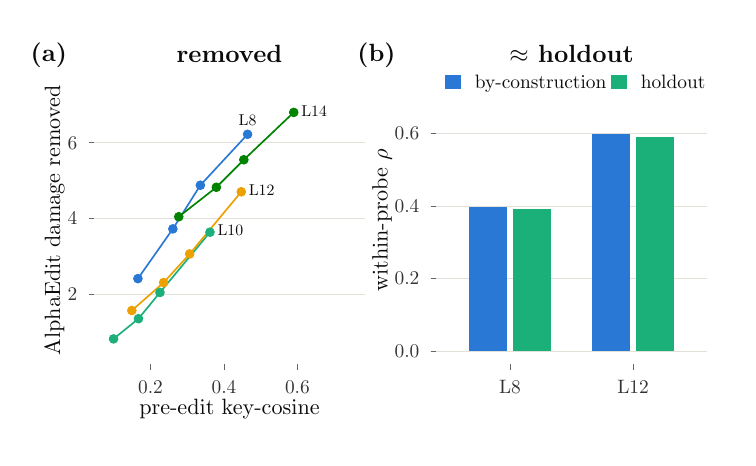
\begin{tikzpicture}[x=1pt,y=1pt]
\definecolor{fillColor}{RGB}{255,255,255}
\path[use as bounding box,fill=fillColor,fill opacity=0.00] (0,0) rectangle (252.94,148.15);
\begin{scope}
\path[clip] (  0.00,  0.00) rectangle (252.94,148.15);
\definecolor{drawColor}{RGB}{255,255,255}
\definecolor{fillColor}{RGB}{255,255,255}

\path[draw=drawColor,line width= 0.6pt,line join=round,line cap=round,fill=fillColor] (  0.00,  0.00) rectangle (252.94,148.15);
\end{scope}
\begin{scope}
\path[clip] (  5.50,  5.50) rectangle (123.85,142.65);
\definecolor{fillColor}{RGB}{255,255,255}

\path[fill=fillColor] (  5.50,  5.50) rectangle (123.85,142.65);
\end{scope}
\begin{scope}
\path[clip] (123.85,  5.50) rectangle (247.44,142.65);
\definecolor{fillColor}{RGB}{255,255,255}

\path[fill=fillColor] (123.85,  5.50) rectangle (247.44,142.65);
\end{scope}
\begin{scope}
\path[clip] ( 23.99, 26.56) rectangle (121.85,130.43);
\definecolor{drawColor}{RGB}{225,224,217}

\path[draw=drawColor,line width= 0.3pt,line join=round] ( 23.99, 51.81) --
	(121.85, 51.81);

\path[draw=drawColor,line width= 0.3pt,line join=round] ( 23.99, 79.18) --
	(121.85, 79.18);

\path[draw=drawColor,line width= 0.3pt,line join=round] ( 23.99,106.55) --
	(121.85,106.55);
\definecolor{drawColor}{RGB}{42,120,214}

\path[draw=drawColor,line width= 0.6pt,line join=round] ( 39.83, 57.47) --
	( 52.46, 75.44) --
	( 62.40, 91.21) --
	( 79.46,109.62);
\definecolor{drawColor}{RGB}{27,175,122}

\path[draw=drawColor,line width= 0.6pt,line join=round] ( 31.03, 35.69) --
	( 40.03, 42.99) --
	( 47.81, 52.47) --
	( 65.88, 74.25);
\definecolor{drawColor}{RGB}{237,161,0}

\path[draw=drawColor,line width= 0.6pt,line join=round] ( 37.64, 45.95) --
	( 49.12, 56.03) --
	( 58.54, 66.39) --
	( 77.18, 88.84);
\definecolor{drawColor}{RGB}{0,131,0}

\path[draw=drawColor,line width= 0.6pt,line join=round] ( 54.60, 79.83) --
	( 68.18, 90.47) --
	( 78.11,100.42) --
	( 96.14,117.53);
\definecolor{drawColor}{RGB}{42,120,214}
\definecolor{fillColor}{RGB}{42,120,214}

\path[draw=drawColor,line width= 0.3pt,line join=round,line cap=round,fill=fillColor] ( 39.83, 57.47) circle (  1.58);

\path[draw=drawColor,line width= 0.3pt,line join=round,line cap=round,fill=fillColor] ( 52.46, 75.44) circle (  1.58);

\path[draw=drawColor,line width= 0.3pt,line join=round,line cap=round,fill=fillColor] ( 62.40, 91.21) circle (  1.58);

\path[draw=drawColor,line width= 0.3pt,line join=round,line cap=round,fill=fillColor] ( 79.46,109.62) circle (  1.58);
\definecolor{drawColor}{RGB}{27,175,122}
\definecolor{fillColor}{RGB}{27,175,122}

\path[draw=drawColor,line width= 0.3pt,line join=round,line cap=round,fill=fillColor] ( 31.03, 35.69) circle (  1.58);

\path[draw=drawColor,line width= 0.3pt,line join=round,line cap=round,fill=fillColor] ( 40.03, 42.99) circle (  1.58);

\path[draw=drawColor,line width= 0.3pt,line join=round,line cap=round,fill=fillColor] ( 47.81, 52.47) circle (  1.58);

\path[draw=drawColor,line width= 0.3pt,line join=round,line cap=round,fill=fillColor] ( 65.88, 74.25) circle (  1.58);
\definecolor{drawColor}{RGB}{237,161,0}
\definecolor{fillColor}{RGB}{237,161,0}

\path[draw=drawColor,line width= 0.3pt,line join=round,line cap=round,fill=fillColor] ( 37.64, 45.95) circle (  1.58);

\path[draw=drawColor,line width= 0.3pt,line join=round,line cap=round,fill=fillColor] ( 49.12, 56.03) circle (  1.58);

\path[draw=drawColor,line width= 0.3pt,line join=round,line cap=round,fill=fillColor] ( 58.54, 66.39) circle (  1.58);

\path[draw=drawColor,line width= 0.3pt,line join=round,line cap=round,fill=fillColor] ( 77.18, 88.84) circle (  1.58);
\definecolor{drawColor}{RGB}{0,131,0}
\definecolor{fillColor}{RGB}{0,131,0}

\path[draw=drawColor,line width= 0.3pt,line join=round,line cap=round,fill=fillColor] ( 54.60, 79.83) circle (  1.58);

\path[draw=drawColor,line width= 0.3pt,line join=round,line cap=round,fill=fillColor] ( 68.18, 90.47) circle (  1.58);

\path[draw=drawColor,line width= 0.3pt,line join=round,line cap=round,fill=fillColor] ( 78.11,100.42) circle (  1.58);

\path[draw=drawColor,line width= 0.3pt,line join=round,line cap=round,fill=fillColor] ( 96.14,117.53) circle (  1.58);
\definecolor{drawColor}{RGB}{11,11,11}

\node[text=drawColor,anchor=base,inner sep=0pt, outer sep=0pt, scale=  0.57] at ( 79.46,112.96) {L8};

\node[text=drawColor,anchor=base west,inner sep=0pt, outer sep=0pt, scale=  0.57] at ( 68.63, 72.95) {L10};

\node[text=drawColor,anchor=base west,inner sep=0pt, outer sep=0pt, scale=  0.57] at ( 79.93, 87.54) {L12};

\node[text=drawColor,anchor=base west,inner sep=0pt, outer sep=0pt, scale=  0.57] at ( 98.89,116.23) {L14};
\end{scope}
\begin{scope}
\path[clip] (  0.00,  0.00) rectangle (252.94,148.15);
\definecolor{drawColor}{gray}{0.20}

\node[text=drawColor,anchor=base east,inner sep=0pt, outer sep=0pt, scale=  0.70] at ( 17.94, 49.53) {2};

\node[text=drawColor,anchor=base east,inner sep=0pt, outer sep=0pt, scale=  0.70] at ( 17.94, 76.90) {4};

\node[text=drawColor,anchor=base east,inner sep=0pt, outer sep=0pt, scale=  0.70] at ( 17.94,104.27) {6};
\end{scope}
\begin{scope}
\path[clip] (  0.00,  0.00) rectangle (252.94,148.15);
\definecolor{drawColor}{gray}{0.40}

\path[draw=drawColor,line width= 0.3pt,line join=round] ( 21.99, 51.81) --
	( 23.99, 51.81);

\path[draw=drawColor,line width= 0.3pt,line join=round] ( 21.99, 79.18) --
	( 23.99, 79.18);

\path[draw=drawColor,line width= 0.3pt,line join=round] ( 21.99,106.55) --
	( 23.99,106.55);
\end{scope}
\begin{scope}
\path[clip] (  0.00,  0.00) rectangle (252.94,148.15);
\definecolor{drawColor}{gray}{0.40}

\path[draw=drawColor,line width= 0.3pt,line join=round] ( 44.37, 24.56) --
	( 44.37, 26.56);

\path[draw=drawColor,line width= 0.3pt,line join=round] ( 70.93, 24.56) --
	( 70.93, 26.56);

\path[draw=drawColor,line width= 0.3pt,line join=round] ( 97.48, 24.56) --
	( 97.48, 26.56);
\end{scope}
\begin{scope}
\path[clip] (  0.00,  0.00) rectangle (252.94,148.15);
\definecolor{drawColor}{gray}{0.20}

\node[text=drawColor,anchor=base,inner sep=0pt, outer sep=0pt, scale=  0.70] at ( 44.37, 15.96) {0.2};

\node[text=drawColor,anchor=base,inner sep=0pt, outer sep=0pt, scale=  0.70] at ( 70.93, 15.96) {0.4};

\node[text=drawColor,anchor=base,inner sep=0pt, outer sep=0pt, scale=  0.70] at ( 97.48, 15.96) {0.6};
\end{scope}
\begin{scope}
\path[clip] (  0.00,  0.00) rectangle (252.94,148.15);
\definecolor{drawColor}{RGB}{11,11,11}

\node[text=drawColor,anchor=base,inner sep=0pt, outer sep=0pt, scale=  0.80] at ( 72.92,  8.23) {pre-edit key-cosine};
\end{scope}
\begin{scope}
\path[clip] (  0.00,  0.00) rectangle (252.94,148.15);
\definecolor{drawColor}{RGB}{11,11,11}

\node[text=drawColor,rotate= 90.00,anchor=base,inner sep=0pt, outer sep=0pt, scale=  0.80] at ( 11.71, 78.50) {AlphaEdit damage removed};
\end{scope}
\begin{scope}
\path[clip] (  0.00,  0.00) rectangle (252.94,148.15);
\definecolor{drawColor}{RGB}{11,11,11}

\node[text=drawColor,anchor=base,inner sep=0pt, outer sep=0pt, scale=  0.90] at ( 72.92,135.45) {\bfseries removed};
\end{scope}
\begin{scope}
\path[clip] (  0.00,  0.00) rectangle (252.94,148.15);
\definecolor{drawColor}{RGB}{11,11,11}

\node[text=drawColor,anchor=base,inner sep=0pt, outer sep=0pt, scale=  0.90] at (  7.65,135.85) {\bfseries (a)};
\end{scope}
\begin{scope}
\path[clip] (147.59, 26.56) rectangle (245.44,130.43);
\definecolor{drawColor}{RGB}{225,224,217}

\path[draw=drawColor,line width= 0.3pt,line join=round] (147.59, 31.28) --
	(245.44, 31.28);

\path[draw=drawColor,line width= 0.3pt,line join=round] (147.59, 57.51) --
	(245.44, 57.51);

\path[draw=drawColor,line width= 0.3pt,line join=round] (147.59, 83.74) --
	(245.44, 83.74);

\path[draw=drawColor,line width= 0.3pt,line join=round] (147.59,109.97) --
	(245.44,109.97);
\definecolor{fillColor}{RGB}{42,120,214}

\path[fill=fillColor] (159.37, 31.28) rectangle (173.16, 83.34);
\definecolor{fillColor}{RGB}{27,175,122}

\path[fill=fillColor] (175.39, 31.28) rectangle (189.18, 82.50);
\definecolor{fillColor}{RGB}{42,120,214}

\path[fill=fillColor] (203.86, 31.28) rectangle (217.64,109.55);
\definecolor{fillColor}{RGB}{27,175,122}

\path[fill=fillColor] (219.87, 31.28) rectangle (233.66,108.70);
\end{scope}
\begin{scope}
\path[clip] (  0.00,  0.00) rectangle (252.94,148.15);
\definecolor{drawColor}{gray}{0.20}

\node[text=drawColor,anchor=base east,inner sep=0pt, outer sep=0pt, scale=  0.70] at (141.54, 29.01) {0.0};

\node[text=drawColor,anchor=base east,inner sep=0pt, outer sep=0pt, scale=  0.70] at (141.54, 55.23) {0.2};

\node[text=drawColor,anchor=base east,inner sep=0pt, outer sep=0pt, scale=  0.70] at (141.54, 81.46) {0.4};

\node[text=drawColor,anchor=base east,inner sep=0pt, outer sep=0pt, scale=  0.70] at (141.54,107.69) {0.6};
\end{scope}
\begin{scope}
\path[clip] (  0.00,  0.00) rectangle (252.94,148.15);
\definecolor{drawColor}{gray}{0.40}

\path[draw=drawColor,line width= 0.3pt,line join=round] (145.59, 31.28) --
	(147.59, 31.28);

\path[draw=drawColor,line width= 0.3pt,line join=round] (145.59, 57.51) --
	(147.59, 57.51);

\path[draw=drawColor,line width= 0.3pt,line join=round] (145.59, 83.74) --
	(147.59, 83.74);

\path[draw=drawColor,line width= 0.3pt,line join=round] (145.59,109.97) --
	(147.59,109.97);
\end{scope}
\begin{scope}
\path[clip] (  0.00,  0.00) rectangle (252.94,148.15);
\definecolor{drawColor}{gray}{0.40}

\path[draw=drawColor,line width= 0.3pt,line join=round] (174.28, 24.56) --
	(174.28, 26.56);

\path[draw=drawColor,line width= 0.3pt,line join=round] (218.76, 24.56) --
	(218.76, 26.56);
\end{scope}
\begin{scope}
\path[clip] (  0.00,  0.00) rectangle (252.94,148.15);
\definecolor{drawColor}{gray}{0.20}

\node[text=drawColor,anchor=base,inner sep=0pt, outer sep=0pt, scale=  0.70] at (174.28, 15.96) {L8};

\node[text=drawColor,anchor=base,inner sep=0pt, outer sep=0pt, scale=  0.70] at (218.76, 15.96) {L12};
\end{scope}
\begin{scope}
\path[clip] (  0.00,  0.00) rectangle (252.94,148.15);
\definecolor{drawColor}{RGB}{11,11,11}

\node[text=drawColor,rotate= 90.00,anchor=base,inner sep=0pt, outer sep=0pt, scale=  0.80] at (130.06, 78.50) {within-probe $\rho$};
\end{scope}
\begin{scope}
\path[clip] (  0.00,  0.00) rectangle (252.94,148.15);
\definecolor{fillColor}{RGB}{42,120,214}

\path[fill=fillColor] (150.68,126.01) rectangle (156.52,130.92);
\end{scope}
\begin{scope}
\path[clip] (  0.00,  0.00) rectangle (252.94,148.15);
\definecolor{fillColor}{RGB}{27,175,122}

\path[fill=fillColor] (210.62,126.01) rectangle (216.46,130.92);
\end{scope}
\begin{scope}
\path[clip] (  0.00,  0.00) rectangle (252.94,148.15);
\definecolor{drawColor}{RGB}{11,11,11}

\node[text=drawColor,anchor=base west,inner sep=0pt, outer sep=0pt, scale=  0.70] at (161.60,126.19) {by-construction};
\end{scope}
\begin{scope}
\path[clip] (  0.00,  0.00) rectangle (252.94,148.15);
\definecolor{drawColor}{RGB}{11,11,11}

\node[text=drawColor,anchor=base west,inner sep=0pt, outer sep=0pt, scale=  0.70] at (221.54,126.19) {holdout};
\end{scope}
\begin{scope}
\path[clip] (  0.00,  0.00) rectangle (252.94,148.15);
\definecolor{drawColor}{RGB}{11,11,11}

\node[text=drawColor,anchor=base,inner sep=0pt, outer sep=0pt, scale=  0.90] at (196.52,135.45) {\bfseries $\approx$ holdout};
\end{scope}
\begin{scope}
\path[clip] (  0.00,  0.00) rectangle (252.94,148.15);
\definecolor{drawColor}{RGB}{11,11,11}

\node[text=drawColor,anchor=base,inner sep=0pt, outer sep=0pt, scale=  0.90] at (126.05,135.85) {\bfseries (b)};
\end{scope}
\end{tikzpicture}
